\definecolor{orange}{RGB}{255,127,0}

\newcommand{\TODO}[1]{\colorbox{orange}{TODO: #1}}
\newcommand{\derives}[1]{\implies \hskip -0.7em ^#1 \hskip 0.7em}







\newpage
\section{Programovací jazyky a překladače}
\begin{pozadavky}
\begin{pitemize}
\item Struktura kompilátoru a navazujících nástrojů (linkery, loadery, debuggery, knihovny, preprocesory).
\item Konečné automaty a lexikální analýza.
\item Syntaktická analýza - LL, LR techniky.
\item Syntaxí řízený překlad a atributové gramatiky.
\item Reprezentace programu mezikódem.
\item Překlad výrazů a programových struktur.
\item Rozsahy platnosti proměnných, aktivační záznamy, implementace vnořených procedur, volací konvence.
\item Vliv architektury počítače na generování kódu a optimalizaci.
\item Metody generování kódu, přidělování registrů, scheduling, optimalizace.
\item Podpora kompilátorů pro synchronizační primitiva, vlákna.
\item Objektově orientované jazyky a principy jejich implementace.
\item Překladače vs. interpretry, skriptovací jazyky.
\end{pitemize}
\end{pozadavky}

\subsection{Struktura kompilátoru a navazujících nástrojů (linkery, loadery, debuggery, knihovny, preprocesory).}

\begin{figure}[h]
	\centering
	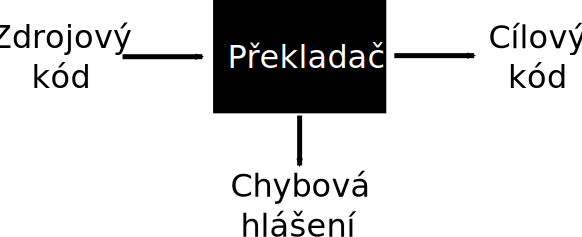
\includegraphics[width=8cm]{i2/softwarove_inzenyrstvi/obrazky/Prekladac-cerna_skrinka.pdf}
	\caption{Překladač jako černá skříňka.}
	\label{pic:Prekladac-cerna_skrinka}
\end{figure}
\begin{definiceN}{Překladač}
Mějme vstupní jazyk \(L_{in}\) generovaný gramatikou \(G_{in}\).
Dále mějme výstupní jazyk \(L_{out}\) generovaný gramatikou \(G_{out}\) nebo přijímaný automatem \(A_{out}\).
\emph{Překladač} je zobrazení \(L_{in} \to L_{out}\), kde \(\forall w_{in} \in L_{in} \exists w_{out} \in L_{out}\) a zároveň pro \(w_{in} \notin L_{in}\) zobrazení neexistuje.
\end{definice}


\subsubsection{Příklady užití technik překladačů}
\begin{pitemize}
	\item Zvýrazňování syntaxe v editorech,
	\item pretty-printer,
	\item statické kontroly kódu,
	\item interpretery,
	\item překladače modelovacích jazyků,
	\item dotazovací jazyky (SQL).
\end{pitemize}


\subsubsection{Historie a srovnání metod tvorby a spouštění programů}
Následující části jsou dobře rozkreslené na slajdech (od p. Bednárka) z C++.

Nejdříve (~1940) se programovalo přímo v binárním kódu, tedy přesně v tom, čemu rozuměl procesor. Později (~1950) byl vymyšlen assembler, tedy jazyk, který zcela přesně popisoval co bude procesor dělat, ale v lidsky čitelnější podobě (do podoby čitelné procesorem se dostane jak jinak než překladačem). Také se v počítačích objevil operační systém, takže se nespouštěl přímo program, ale nejprve se spustil OS a ten teprve (pomocí loaderu) načetl do paměti program a spustil jej. Program tedy už nemusel být ve formátu, kterému rozumí přímo procesor, ale mohl být obalen dalšími informacemi, které rozpoznával a zpracovával operační systém. Potom se objevily jazyky na vyšší úrovni, které se do spustitelného souboru kompilovaly a tyto jazyky byly vyšší a vyšší.

Další možností spouštění programů je jejich interpretace, tedy vlastně spojení kompilace a spouštění. Program je řádku po řádce parsován a prováděn. Běh takového programu je však pomalý, což se dá vyřešit tak, že program se nejprve (při spouštění) přeloží do mezikódu a ten je teprve interpretován (mezikód je přinejmenším menší). Překlad se ale dělá při každém spuštění, což je neefektivní. Překlad (do mezikódu) se může udělat jen jednou a vytvořit tak jakýsi soubor spustitelný pomocí interpretru. Výhodou (oproti klasickému překladu přímo do binární podoby, které rozumí CPU) je platformní nezávislost mezikódu. Stačí aby pro daný procesor existoval interpret a je možné mezikód na tomto procesoru spustit. Opět se však potýkáme s neefektivitou interpretace mezikódu. Jako řešení byl vymyšlen tzv. JIT (Just in time compiler), který mezikód za běhu programu překládá do strojového kódu a ten teprve spouští. Výhodou je, že pokud se nějaká část programu provádí znovu, tak ji stačí jen spustit a už není potřeba mezikód.

Poznámka: Dnešní překladače již většinou vygenerují optimálnější kód než by člověk dokázal napsat.

\begin{table}[h]
	{\centering
	\begin{tabular}{ l || p{4cm} | p{4cm} }
		& JIT & Klasika \\
		\hline
		\hline
		Distribuce & bytecode & binární instrukce \\
		\hline
		Závislost distribuce & jazyk a překladač & procesor a OS \\
		\hline
		Výhoda překladače & překladač zná přesně cílový procesor, může sledovat chování programu & překladač má hodně času na překlad
	\end{tabular} \\
	}
	\caption{Srovnání klasické metody kompilace a JIT}
	\label{tab:Srovnani_JIT}
\end{table}


\subsubsection{Klasická kompilace}
\begin{figure}[h]
	\centering
	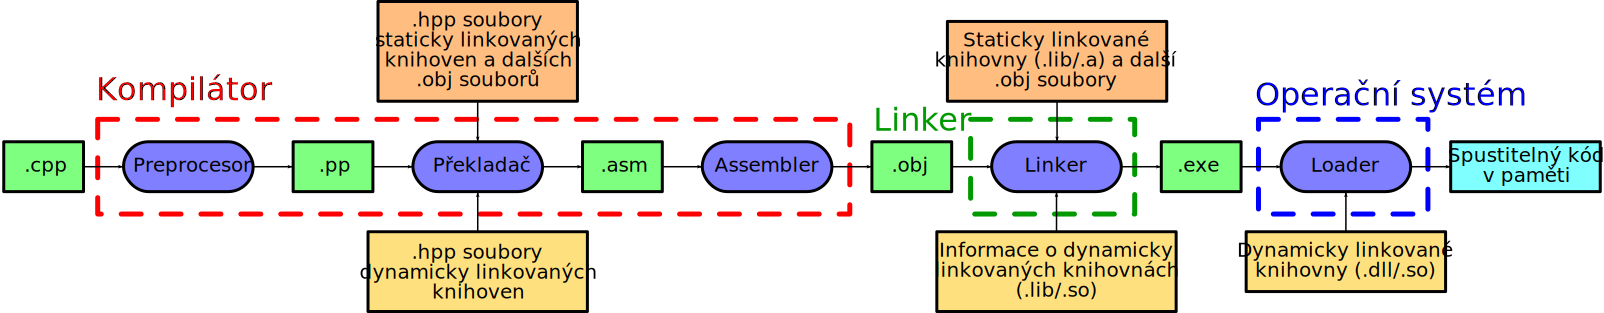
\includegraphics[width=15cm]{i2/softwarove_inzenyrstvi/obrazky/Preklad.pdf}
	\caption{Průběh překladu zdrojových kódů v C++.}
	\label{pic:Preklad}
\end{figure}

Všimněte si, že to, co se běžně nazývá překladačem je vlastně složeno z několika menších překladačů (preprocesor, překladač, assembler).

\paragraph{Překladač}
Na obrázku \ref{pic:Preklad} je červeně vyznačena oblast, kterou má na starosti program, který je běžně označován jako \emph{překladač} či \emph{kompilátor}. Tento program tedy provádí překlad ze zdrojových kódů do binárních souborů (za pomoci hlavičkových souborů). Tento program poběží tolikrát, kolik je v kompilovaném projektu kódu (.cpp). Pokud je v souboru .cpp odkaz na něco (proměnnou, funkci aj.) z jiného .cpp nebo z knihovny, tak na daném místě překladač nechá volné místo pro doplnění adresy (musí vědět kolik místa nechat -- proto potřebuje hlavičkové soubory odkazovaných souborů a knihoven).

\paragraph{Linker}
Jednotlivé soubory .obj, které vytvoří překladač je ještě potřeba spojit do jednoho spustitelného souboru. To má na starosti tzv. linker, který je spojí a doplní adresy do prázdných míst, které tam nechal překladač. Nemůže však vyplnit místa pro dynamicky linkované knihovny, proto je opět nechá prázdná.

\paragraph{Loader}
Hlavním úkolem loaderu je načíst program do paměti a spustit ho. Před jeho spuštěním je však potřeba přilinkovat ještě dynamicky linkované knihovny, takže loader vyplní prázdná místa, která mu tam nechal linker. Dynamické linkování se dá dělat několika způsoby. Buď se vyplní rovnou všechny adresy na všech místech, kde se program odkazuje do knihovny (těch ale může být hodně), nebo se do knihovny neadresuje přímo, ale přičítá se její offset a loader vyplní jen tento offset. Druhá možnost má nevýhodu v tom, že při každém volání se musí zjistit offset a ten se ještě musí přičíst k adrese v knihovně. Dá se tedy udělat kompromis, totiž že se udělá tabulka (používaných) adres v knihovně, kterou loader vyplní. V tabulce nejsou duplicity, takže vyplnění nebude trvat tak dlouho a při volání se nemusí nic sčítat, pouze se provede dereference. Která možnost se použije samozřejmě nemůže rozhodovat sám loader (potřebuje aby mu vhodné struktury připravil už překladač).

\paragraph{Debugger}
K ladění programů slouží debugger, který používá jak zkompilovaný program, tak zdrojové kódy. Potřebuje se však nějak dozvědět, která část zkompilovaného programu odpovídá které části zdrojových kódů. Tuto informaci mu poskytuje překladač.

\paragraph{Knihovny}
Knihovny se dělí na statické a dynamické. Statické knihovny se linkují s programem za kompilace (linkerem) a dynamické se linkují před spuštěním (loaderem). Způsoby linkování dynamických knihoven viz část o loaderu. Dynamické knihovny lze navíc načítat až za běhu aplikace. Knihovna tak může být načtena do paměti až v případě potřeby.

\paragraph{Preprocesor}
Zvláštní částí kompilátoru je preprocesor, což je vlastně sám překladač. Překládá totiž kód z jazyka preprocesoru do jazyka C/C++/... Z možností preprocesoru jazyka C se nejčastěji používá podmíněný překlad, jehož použití je vidět na ukázce kódu \ref{cod:Preprocesor}. V jazyce C se preprocesor používal více (např. pro konstanty), v C++ již byly některá tato použití nahrazena možnostmi samotného jazyka C++.
\begin{kod}[h]
	\begin{verbatim}
		#ifdef unix
		  std::cout << "Ahoj unixáku!";
		#else
		  std::cout << "Ahoj neunixáku!";
		#endif
	\end{verbatim}
	\caption{Příklad použití preprocesoru.}
	\label{cod:Preprocesor}
\end{kod}


\subsubsection{Struktura překladače}
\begin{figure}[h]
	\centering
	\includegraphics[width=15cm]{i2/softwarove_inzenyrstvi/obrazky/Faze_prekladu.png}
	\caption{Fáze překladu.}
	\label{pic:Prekladac-cerna_skrinka}
\end{figure}
Překladač se skládá z front endu a back endu. Překlad probíhá v několika fázích. Budeme předpokládat syntaxí řízený překlad. Překlad začíná spuštěním syntaktického analyzátoru, který postupně žádá lexikální analyzátor o další token. Ze získaných tokenů se snaží \uv{složit} některé z pravidel gramatiky (buď shora dolů nebo naopak). Jakmile jej najde, proběhne sémantická analýza, která podle pravidla upraví tabulky symbolů a případně proběhne generování mezikódu. Jakmile je dokončeno generování mezikódu, mohou na něm proběhnout optimalizace. Mezikód se potom předá back endu, který z něj vygeneruje kód na kterém může opět provést další (platformě specifické) optimalizace. Pokud se během celého procesu objeví chyba, překladač by se ji měl pokusit nějakým způsobem ignorovat (ale nahlásit) a pokračovat dál pokud možno tak, aby tím nevznikly další domnělé chyby a zároveň aby se na žádnou chybu nezapomnělo.




\subsection{Konečné automaty a lexikální analýza.}

\TODO{Dopsat tuto otázku: Co mají konečné automaty společného s lexikální analýzou?}




\subsection{Syntaktická analýza - LL, LR techniky.}

\begin{figure}[h]
	\centering
	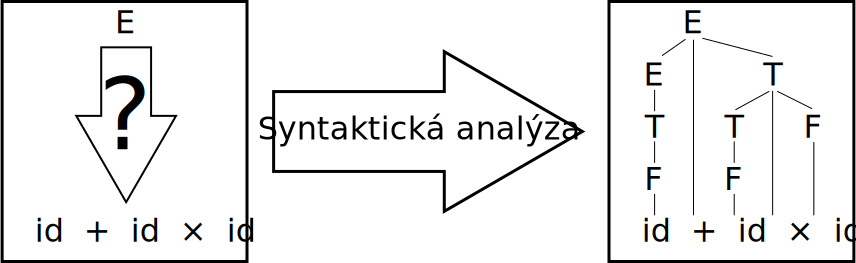
\includegraphics[width=8cm]{i2/softwarove_inzenyrstvi/obrazky/Syntakticka_analyza.pdf}
	\caption{Hlavní úkol syntaktické analýzy.}
	\label{pic:Syntakticka_analyza}
\end{figure}

Hlavním úkolem syntaktické analýzy je rozpoznat, jestli slovo (=zdrojový kód) na vstupu je slovem ze vstupního jazyka (=korektním programem v daném jazyce) a vyrobí jeho derivační strom.

Používá-li se technika syntaxí řízeného překladu, syntaktická analýza řídí celý překladač (rozuměj hlavní cyklus překladače je v syntaktickém analyzátoru).

\begin{figure}[h]
	\centering
	\includegraphics[width=13cm]{i2/softwarove_inzenyrstvi/obrazky/Syntakticka_analyza_v_prekladaci.png}
	\caption{Syntaktická analýza ve vztahu k ostatním částem překladače.}
	\label{pic:Syntakticka_analyza_v_prekladaci}
\end{figure}

Na obrázku \ref{pic:Syntakticka_analyza_v_prekladaci} je vidět propojení mezi syntaktickou analýzou a tabulkou symbolů, které by správně nemělo být potřeba, ale využívá se k obejití některých kontextových vlastností jazyka.

Je-li řeč o bezkontextových gramatikách, což běžné jazyky (přibližně) splňují, je potřeba zásobníkový automat, který postaví derivační strom. Vlastnosti jazyka, které přesahují bezkontextovost (např. deklarace identifikátoru před použitím nebo stejný počet parametrů v deklaraci a volání funkce) jsou potom řešeny při sémantické analýze.

\begin{definice}
	Znak nazveme \emph{symbolem}, je-li tento znak terminálem nebo neterminálem.
\end{definice}


\subsubsection{Jednoznačnost gramatiky}

Ke každému slovu musí být derivační strom určen jednoznačně. Případem situace, kdy tomu tak nemusí být a je třeba gramatiku upravit (oproti přirozené verzi), je problém \uv{dangling else}, kdy podle (přirozené) gramatiky nevíme, ke kterému \uv{ifu} větev else patří.

\begin{kod}[h]
	\begin{verbatim}
		stmt -> if expr then stmt
		      | if expr then stmt else stmt
		      | while expr do stmt
		      | goto num
	\end{verbatim}
	\caption{Původní (přirozená) gramatika.}
	\label{cod:Prirozena_gramatika}
\end{kod}

\begin{kod}[h]
	\begin{verbatim}
		stmt -> hodny_stmt
		      | zly_stmt
		hodny_stmt -> if expr then hodny_stmt else hodny_stmt
		      | while expr do hodny_stmt
		      | goto num
		zly_stmt -> if expr then zly_stmt
		      | if expr then hodny_stmt else zly_stmt
		      | while expr do lzy_stmt
	\end{verbatim}
	\caption{Jednoznačná gramatika.}
	\label{cod:Jednoznacna_gramatika}
\end{kod}

V ukázkách kódu \ref{cod:Prirozena_gramatika} a \ref{cod:Jednoznacna_gramatika} \uv{while} reprezentuje všechny příkazy, které mají na konci \uv{stmt} a \uv{goto} reprezentuje všechny příkazy, které na konci \uv{stmt} nemají.


\subsubsection{Levá rekurze}

Dalším problémem pro syntaktickou analýzu, pokud dělá analýzu shora dolů, je levá rekurze.

\begin{definice}
	Řekneme, že gramatika je \emph{levě rekurzivní}, pokud obsahuje neterminál \(A\), pro který platí, \(A \derives{+} A \alpha\), kde \(\alpha\) je nějaký řetězec symbolů. Tedy \(A\) se dá pomocí pravidel gramatiky převést na \(A\alpha\). Příklad odstranění levé rekurze je vidět na ukázce kódu \ref{cod:Odstraneni_rekurze}.
\end{definice}

\begin{kod}[h]
	Původní gramatika
	\begin{verbatim}
		A -> Aa
		A -> b
	\end{verbatim}
	
	Nová gramatika
	\begin{verbatim}
		A -> bB
		B -> aB
		B -> {lambda}
	\end{verbatim}
	\caption{Odstranění levé rekurze.}
	\label{cod:Odstraneni_rekurze}
\end{kod}


\subsubsection{Levá faktorizace}

V gramatice se může objevit také tzv. levá faktorizace, což je situace, kdy máme k dispozici dvě pravidla, ale podle prvního neterminálu si nedokážeme vybrat, které použít. Řešení je jednoduché: Vytvořit nové pravidlo, které bude obsahovat začátek a teprve v místě kde se původní pravidla lišila bude další neterminál. Konkrétní řešení ukazuje kód \ref{cod:Odstraneni_faktorizace}.

\begin{kod}[h]
	Původní gramatika
	\begin{verbatim}
		A -> ab
		A -> ac
	\end{verbatim}
	
	Nová gramatika
	\begin{verbatim}
		A -> aB
		B -> b
		B -> c
	\end{verbatim}
	\caption{Odstranění levé faktorizace.}
	\label{cod:Odstraneni_faktorizace}
\end{kod}


\subsubsection{Postup syntaktické analýzy}

Syntaktická analýza může probíhat dvěma směry, a to buď shora dolů nebo zdola nahoru.

\paragraph{Shora dolů} Při analýza shora dolů se analyzátor snaží určit použitá pravidla v derivačním stromě od jeho kořene (a z levé strany). Tento postup lze realizovat buď rekurzivním sestupem (obvyklejší) nebo pomocí LL automatu. Analýza shora dolů najde nejlevější derivaci.

\paragraph{Zdola nahoru} Naopak analýza zdola nahoru se snaží hledat použitá pravidla zdola nahoru (a z levé strany), tedy derivační strom vytváří tak, že postupně listy spojuje do menších stromů a ty do větších až dostane celý derivační strom. Tento postup lze realizovat LR automatem. \TODO{Překontrolovat/doplnit.}

\paragraph{Názvy gramatik} \TODO{Dopsat.}


\subsubsection{FIRST a FOLLOW}

\begin{definiceN}{FIRST}
	Nechť \(\alpha\) je řetězec symbolů gramatiky, pak \(FIRST(\alpha)\) je množina terminálů, kterými začínají všechny řetězce derivované z \(\alpha\). Pokud \(\alpha\) může derivovat na \(\lambda\), pak je \(\lambda\) také ve \(FIRST(\alpha)\).
\end{definiceN}

\begin{definiceN}{FOLLOW}
	Nechť \(A\) je neterminál, potom \(FOLLOW(A)\) definujeme jako množinu terminálů, které se mohou vyskytovat těsně za \(A\) v nějakém řetězci, který vznikl derivací z počátečního neterminálu gramatiky (\(S \derives{*} \alpha A a \beta\), pro nějaké řetězce symbolů \(\alpha\) a \(\beta\)). Pokud je \(A\) nejpravější symbol v nějakém přepisu, pak je ve \(FOLLOW(A)\) i \(\$\) -- speciální symbol.
\end{definiceN}

\begin{priklad}
	Mějme řetězec \(ABC\), kde \(A\), \(B\) i \(C\) jsou neterminály a k tomuto řetězci jsme se dostali pravidlem \(S \to ABC\), které je jediné pro přepis \(S\). Množina \(FIRST(B)\) nám teď říká, jaké neterminály se můžou objevit na začátku řetězce, na který se přepíše neterminál \(B\). Dokonce ve \(FIRST(B)\) jsou i terminály se kterými řetězec v gramatice nemůže skončit. \(FOLLOW(B)\) nám říká, jaké terminály mohou následovat těsně za řetězcem na který se přepíše \(B\). Pokud je použité pravidlo jediné ve kterém se vyskytuje na pravé straně neterminál \(B\), pak \(FOLLOW(B) = FIRST(C)\) (až na \(\lambda\) a \(\$\)).
\end{priklad}

\TODO{Dopsat konstrukci FIRST a FOLLOW.}


\subsubsection{Rekurzivní sestup}

\TODO{Dopsat rekurzivní sestup.}


\subsubsection{LL automat}

\TODO{Dopsat (vč. LL(k) gramatiky).}


\subsubsection{LR automat}

\TODO{Dopsat.}




\subsection{Syntaxí řízený překlad a atributové gramatiky.}
\subsection{Reprezentace programu mezikódem.}
\subsection{Překlad výrazů a programových struktur.}
\subsection{Rozsahy platnosti proměnných, aktivační záznamy, implementace vnořených procedur, volací konvence.}
\subsection{Vliv architektury počítače na generování kódu a optimalizaci.}
\subsection{Metody generování kódu, přidělování registrů, scheduling, optimalizace.}
\subsection{Podpora kompilátorů pro synchronizační primitiva, vlákna.}
\subsection{Objektově orientované jazyky a principy jejich implementace.}
\subsection{Překladače vs. interpretry, skriptovací jazyky.}
